%
% $RCSfile: hierarchy_and_ontology.tex,v $
%
% Copyright (c) 2001-2004. Christian Heller. All rights reserved.
%
% No copying, altering, distribution or any other actions concerning this
% document, except after explicit permission by the author!
% At some later point in time, this document is planned to be put under
% the GNU FDL license. For now, _everything_ is _restricted_ by the author.
%
% http://www.cybop.net
% - Cybernetics Oriented Programming -
%
% http://www.resmedicinae.org
% - Information in Medicine -
%
% @author Christian Heller <christian.heller@tuxtax.de>
%

\section{Hierarchy and Ontology}
\label{hierarchy_and_ontology_heading}

Section \ref{basic_patterns_heading} explained three design patterns that are
widely used in software architectures. It has shown similarities between them
and raised the question if they could possibly be merged into just one pattern,
called \emph{Translator}, what will be described in section
\ref{logical_architecture_heading}.
Yet before, this section will demonstrate how the principle of \emph{Hierarchy}
may be applied to obtain an \emph{Ontology}.

%
% $RCSfile: association_elimination.tex,v $
%
% Copyright (c) 2001-2004. Christian Heller. All rights reserved.
%
% No copying, altering, distribution or any other actions concerning this
% document, except after explicit permission by the author!
% At some later point in time, this document is planned to be put under
% the GNU FDL license. For now, _everything_ is _restricted_ by the author.
%
% http://www.cybop.net
% - Cybernetics Oriented Programming -
%
% http://www.resmedicinae.org
% - Information in Medicine -
%
% @author Christian Heller <christian.heller@tuxtax.de>
%

\subsection{Association Elimination}
\label{association_elimination_heading}

An \emph{Electronic Health Record} (EHR) will serve as example domain model whose class
structure is shown in part in figure \ref{parent_eliminate_child_associations_figure}.
It consists of numerous parts whereof at least two will be of type \emph{Address}
and \emph{Problem}, respectively. Following the \emph{Episode-based EHR}
recommendation \cite{westerhof}, \emph{Problem} may consist of \emph{Subjective}
and \emph{Objective}. All these associations between classes are needed to
navigate through the domain model.

\begin{figure}[ht]
    \begin{center}
        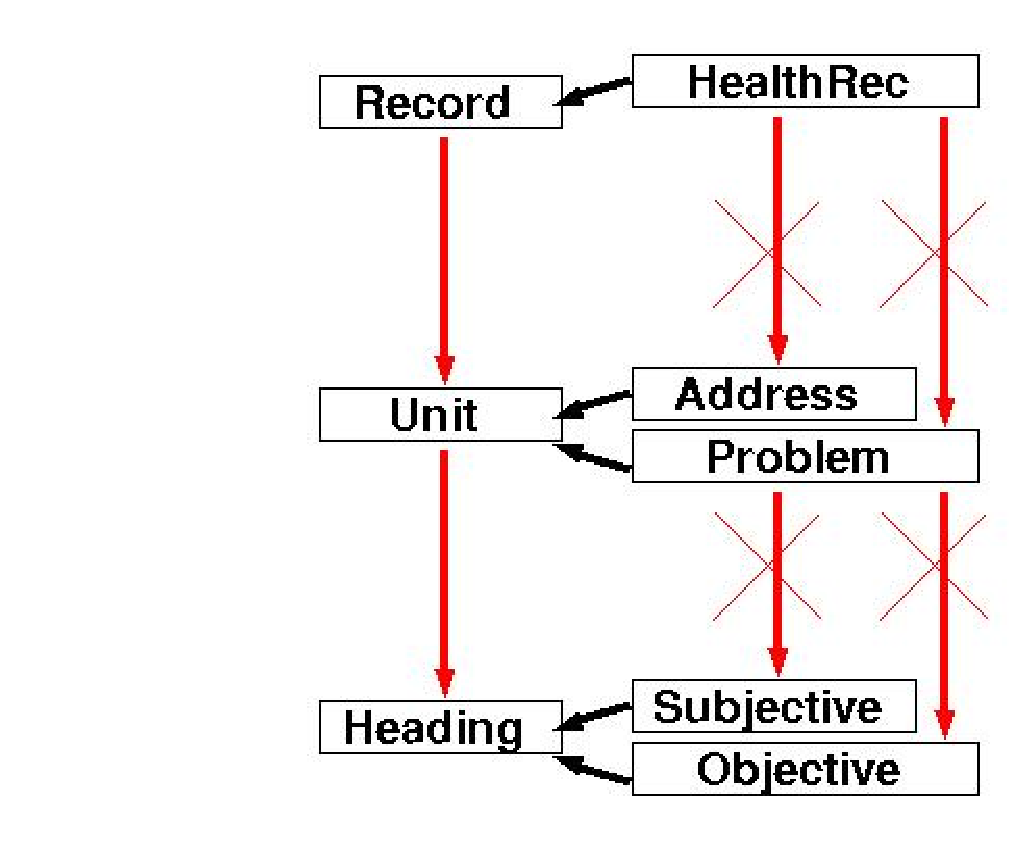
\includegraphics[scale=0.4]{vector/parent_eliminate_child_associations.eps}
        \caption{Parent- eliminate Child Associations}
        \label{parent_eliminate_child_associations_figure}
    \end{center}
\end{figure}

A frequent design decision in object oriented programming is to sum up common
properties of sub classes by introducing a common super class. It is not only
properties, but also the \emph{Granularity} of objects that can lead to the
creation of a super class. The OpenEHR project \cite{openehr} suggests to let
the above-mentioned classes inherit from the more coarse-grained super classes
\emph{Record}, \emph{Unit}, \emph{Heading} and others.\\
Whichever reason -- once the super classes are there, they should be associated
similarly to their sub classes, that is in the same direction, using unidirectional
dependencies. Afterwards, all associations between sub classes become superfluous
as every sub class can reach its sibling across their parent classes' association
(figure \ref{parent_eliminate_child_associations_figure}).\\
Here a short Java code example for how the \emph{HealthRecord} may retrieve a
reference to \emph{Address}:
\begin{verbatim}
Address a = (Address) get("address");
\end{verbatim}
\emph{HealthRecord} inherits the \emph{get} method from its super class \emph{Record}.
\emph{Record} holds many instances of type \emph{Unit} and differing sub types.
The \emph{get} method delivers back an object that still needs to be down-casted
to the expected sub type \emph{Address}.\\
The definition of classes, their dependencies (defined by associations) and granularities
(defined by inheritance) in a software system results in several layers of classes of
common granularity, as shown in figure \ref{ontological_levels_and_item_container_figure}.
These layers are often called \emph{Ontological Level} as they form an \emph{Ontology}
(see section \ref{ontology_heading}).

\begin{figure}[ht]
    \begin{center}
        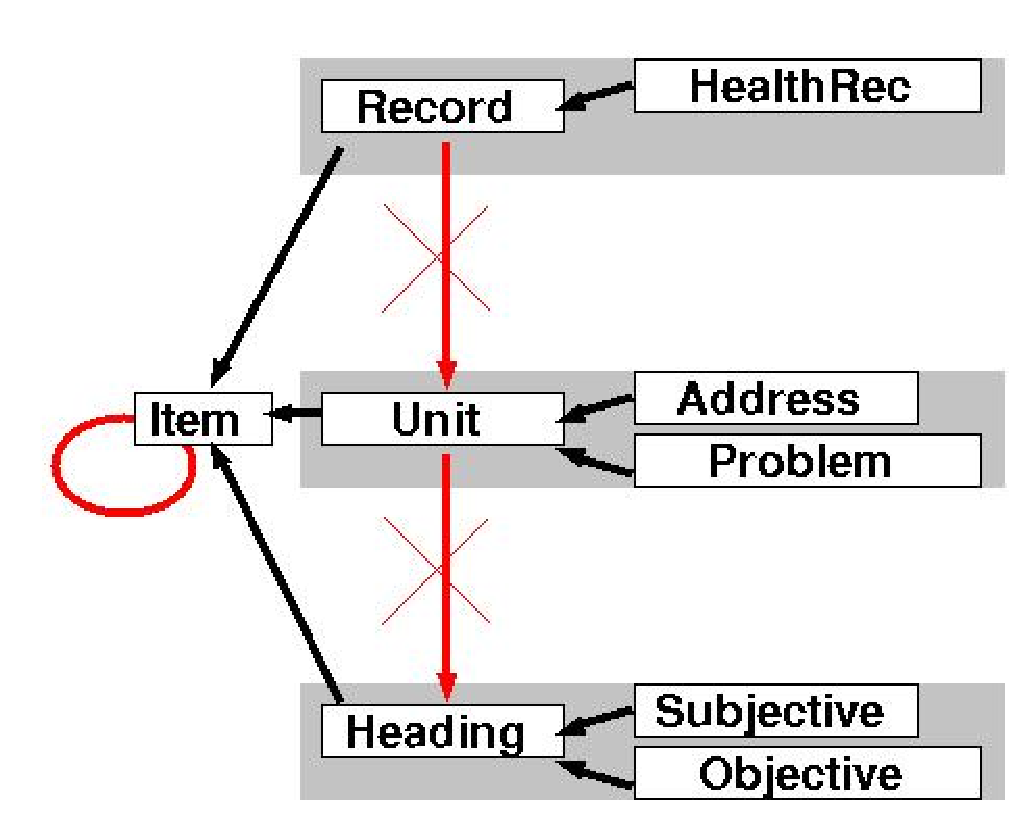
\includegraphics[scale=0.4]{vector/ontological_levels_and_item_container.eps}
        \caption{Ontological Levels and Item Container}
        \label{ontological_levels_and_item_container_figure}
    \end{center}
\end{figure}

Continuing the structure process of introducing more and more common, coarse-grained
or fine-grained super classes, the development culminates in one top-most super
class of all other classes in the system, which this paper calls \emph{Item}.
It is as general as the \emph{java.lang.Object} class for the Java class library,
only that it additionally represents a container that can store objects of any type,
as explained in \cite{hellerbohl}. In other words, \emph{Item} provides the meta
functionality of a container behaviour to \emph{all} other classes.


%
% $RCSfile: ontology.tex,v $
%
% Copyright (c) 2001-2004. Christian Heller. All rights reserved.
%
% No copying, altering, distribution or any other actions concerning this
% document, except after explicit permission by the author!
% At some later point in time, this document is planned to be put under
% the GNU FDL license. For now, _everything_ is _restricted_ by the author.
%
% http://www.cybop.net
% - Cybernetics Oriented Programming -
%
% http://www.resmedicinae.org
% - Information in Medicine -
%
% @author Christian Heller <christian.heller@tuxtax.de>
%

\subsection{Ontology}
\label{ontology_heading}

Manifold definitions of the word \emph{Ontology} exist. They come from philosophy,
metaphysics, information technology and others -- too many to list here.
This document uses its own, adapted definition and considers an ontology to be
\emph{a strict hierarchy of abstract items, organized in levels of growing
granularity, that are solely unidirectionally related}. It such represents a
systematic description of complex domain contexts.

\begin{figure}[ht]
    \begin{center}
        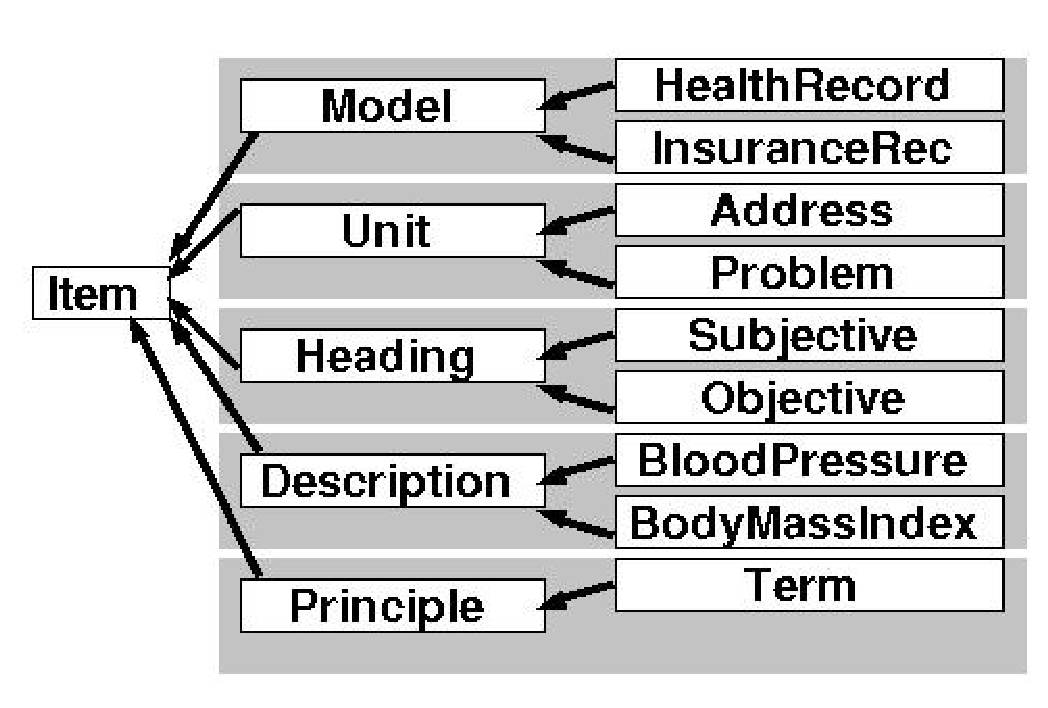
\includegraphics[scale=0.4]{vector/electronic_health_record_ontology.eps}
        \caption{Electronic Health Record Ontology}
        \label{electronic_health_record_ontology_figure}
    \end{center}
\end{figure}

Figure \ref{electronic_health_record_ontology_figure} shows one possible ontology
of an electronic health record, as described in the previous section.



